%********************************************************************
% Appendix
%*******************************************************
% If problems with the headers: get headings in appendix etc. right
%\markboth{\spacedlowsmallcaps{Appendix}}{\spacedlowsmallcaps{Appendix}}
\chapter{Appendix}

\section{Maximal Conductances for Model Neurons}
The dynamics and compartment parameters of each model neuron are described in \autoref{ch:methods}. The maximal conductances are as follows

\begin{table}[h]
	\myfloatalign
	\begin{tabularx}{\textwidth}{ccc} \toprule
		\tableheadline{Current} & $\bar{g}~(\mu\mathrm{S/mm^2})$ & \tableheadline{Notes}\\ \midrule
		\acs{IA} & 1844 & \\
		\acs{ICaS} & 103 & \\
		\acs{IH} & 0.39 &\\
		\acs{IKCa} & 214 & \\
		\acs{IKd} & 1746.96 & \\
		\acs{IMI} & 1 & 0 in the decentralized case \\ \bottomrule
	\end{tabularx}
	\caption{Maximal conductances for \autoref{fig:abwmod}.}
	\label{tab:appendix1}
\end{table}

\begin{table}[h]
	\myfloatalign
	\begin{tabularx}{\textwidth}{cccc} \toprule
		\tableheadline{Current} & \acs{AB}-\acs{PD} $\bar{g}~(\mu\mathrm{S/mm^2})$ & \acs{LP} $\bar{g}~(\mu\mathrm{S/mm^2})$ & \acs{PY} $\bar{g}~(\mu\mathrm{S/mm^2})$ \\ \midrule
		\acs{IA} & 483.25 & 341.98 & 449.88 \\
		\acs{ICaS} & 18.647 & 39.765 & 85.009 \\
		\acs{ICaT} & 30.368 & 14.649 & 9.9027 \\ 
		\acs{IH} & 0.14027 & 0.47477 & 0.3751 \\
		\acs{IKCa} & 99.998 & 88.89 & 14.637 \\
		\acs{IKd} & 1030.1 & 1093 & 1228.2 \\
		\acs{INa} & 1274.5 & 985.64 & 1797.1 \\ \bottomrule
	\end{tabularx}
	\caption{Maximal conductances for \autoref{fig:networkab47traces}.}
	\label{tab:appendix2ionic}
\end{table}

\begin{table}[h]
	\myfloatalign
	\begin{tabularx}{\textwidth}{cccc} \toprule
		\tableheadline{Current} & \tableheadline{Presynaptic} & \tableheadline{Postsynaptic} & $\bar{g}~(\mu\mathrm{S/mm^2})$ \\ \midrule
		\acs{Ichol} & AB-PD & LP & 59.724 \\
		\acs{Ichol} & AB-PD & PY & 94.508 \\
		\acs{Iglut} & AB-PD & LP & 79.803 \\ 
		\acs{Iglut} & AB-PD & PY & 97.881 \\
		\acs{Iglut} & LP & PY & 1.6985 \\
		\acs{Iglut} & PY & LP & 84.74 \\
		\acs{Iglut} & LP & AB-PD & 0.0128\\ \bottomrule
	\end{tabularx}
	\caption{Maximal conductances for \autoref{fig:networkab47traces}.}
	\label{tab:appendix2synaptic}
\end{table}

\begin{table}[h]
	\myfloatalign
	\begin{tabularx}{\textwidth}{cccc} \toprule
		\tableheadline{Current} & \acs{AB}-\acs{PD} $\bar{g}~(\mu\mathrm{S/mm^2})$ & \acs{LP} $\bar{g}~(\mu\mathrm{S/mm^2})$ & \acs{PY} $\bar{g}~(\mu\mathrm{S/mm^2})$ \\ \midrule
		\acs{IA} & 499.57 & 488.85 & 150.95 \\
		\acs{ICaS} & 42.16 & 5.9231 & 100 \\
		\acs{ICaT} & 29.236 & 48.989 & 0.00081 \\ 
		\acs{IH} & 0.3182 & 0.3666 & 0.1264 \\
		\acs{IKCa} & 100 & 62.559 & 99.359 \\
		\acs{IKd} & 878.65 & 911.94 & 816.2 \\
		\acs{INa} & 990.11 & 1733.6 & 1926.2 \\ \bottomrule
	\end{tabularx}
	\caption{Maximal conductances for \autoref{fig:networklp28traces}.}
	\label{tab:appendix3ionic}
\end{table}

\begin{table}[h]
	\myfloatalign
	\begin{tabularx}{\textwidth}{cccc} \toprule
		\tableheadline{Current} & \tableheadline{Presynaptic} & \tableheadline{Postsynaptic} & $\bar{g}~(\mu\mathrm{S/mm^2})$ \\ \midrule
		\acs{Ichol} & AB-PD & LP & 43.589 \\
		\acs{Ichol} & AB-PD & PY & 91.146 \\
		\acs{Iglut} & AB-PD & LP & 46.6953 \\ 
		\acs{Iglut} & AB-PD & PY & 71.918 \\
		\acs{Iglut} & LP & PY & 7.2045 \\
		\acs{Iglut} & PY & LP & 4.0693 \\
		\acs{Iglut} & LP & AB-PD & 43.899 \\ \bottomrule
	\end{tabularx}
	\caption{Maximal conductances for \autoref{fig:networklp28traces}.}
	\label{tab:appendix3synaptic}
\end{table}

\begin{table}[h]
	\myfloatalign
	\begin{tabularx}{\textwidth}{cccc} \toprule
		\tableheadline{Current} & \acs{AB}-\acs{PD} $\bar{g}~(\mu\mathrm{S/mm^2})$ & \acs{LP} $\bar{g}~(\mu\mathrm{S/mm^2})$ & \acs{PY} $\bar{g}~(\mu\mathrm{S/mm^2})$ \\ \midrule
		\acs{IA} & 384.09 & 215.15 & 398.88 \\
		\acs{ICaS} & 4.7276 & 21.739 & 91.294 \\
		\acs{ICaT} & 40.901 & 55.179 & 4.7064 \\ 
		\acs{IH} & 0.26391 & 0.48577 & 0.49937 \\
		\acs{IKCa} & 56.614 & 83.753 & 6.9534 \\
		\acs{IKd} & 766.44 &   1196 & 1103.7 \\
		\acs{INa} & 1719.3 & 1791.4 & 1978.6  \\ \bottomrule
	\end{tabularx}
	\caption{Maximal conductances for \autoref{fig:networkablp14traces}.}
	\label{tab:appendix4ionic}
\end{table}

\begin{table}[h]
	\myfloatalign
	\begin{tabularx}{\textwidth}{cccc} \toprule
		\tableheadline{Current} & \tableheadline{Presynaptic} & \tableheadline{Postsynaptic} & $\bar{g}~(\mu\mathrm{S/mm^2})$ \\ \midrule
		\acs{Ichol} & AB-PD & LP & 0.70694 \\
		\acs{Ichol} & AB-PD & PY & 2.5239 \\
		\acs{Iglut} & AB-PD & LP & 14.382 \\ 
		\acs{Iglut} & AB-PD & PY & 96.992 \\
		\acs{Iglut} & LP & PY & 22.72 \\
		\acs{Iglut} & PY & LP & 16.11 \\
		\acs{Iglut} & LP & AB-PD & 54.05 \\ \bottomrule
	\end{tabularx}
	\caption{Maximal conductances for \autoref{fig:networkablp14traces}.}
	\label{tab:appendix4synaptic}
\end{table}

\begin{table}[h]
	\myfloatalign
	\begin{tabularx}{\textwidth}{cccc} \toprule
		\tableheadline{Current} & \acs{AB}-\acs{PD} $\bar{g}~(\mu\mathrm{S/mm^2})$ & \acs{LP} $\bar{g}~(\mu\mathrm{S/mm^2})$ & \acs{PY} $\bar{g}~(\mu\mathrm{S/mm^2})$ \\ \midrule
		\acs{IA} & 48.274  & 486.59 &  361.85 \\
		\acs{ICaS} & 0.95921 &  52.628 &  35.453 \\
		\acs{ICaT} & 44.247 &  31.541 &  58.985 \\ 
		\acs{IH} & 0.057166 & 0.42321 & 0.42576 \\
		\acs{IKCa} & 63.068 &  93.046 & 54 \\
		\acs{IKd} & 957.19 &  1075.4 &  1153.9 \\
		\acs{INa} & 1584.4 &  1196.8 &  1835.9  \\ \bottomrule
	\end{tabularx}
	\caption{Maximal conductances for \autoref{fig:traces1}.}
	\label{tab:appendix5ionic}
\end{table}

\begin{table}[h]
	\myfloatalign
	\begin{tabularx}{\textwidth}{cccc} \toprule
		\tableheadline{Current} & \tableheadline{Presynaptic} & \tableheadline{Postsynaptic} & $\bar{g}~(\mu\mathrm{S/mm^2})$ \\ \midrule
		\acs{Ichol} & AB-PD & LP & 21.247 \\
		\acs{Ichol} & AB-PD & PY & 17.497 \\
		\acs{Iglut} & AB-PD & LP & 92.692 \\ 
		\acs{Iglut} & AB-PD & PY & 74.007 \\
		\acs{Iglut} & LP & PY & 97.419 \\
		\acs{Iglut} & PY & LP & 93.541 \\
		\acs{Iglut} & LP & AB-PD & 51.799 \\ \bottomrule
	\end{tabularx}
	\caption{Maximal conductances for \autoref{fig:traces1}.}
	\label{tab:appendix5synaptic}
\end{table}

\begin{table}[h]
	\myfloatalign
	\begin{tabularx}{\textwidth}{cccc} \toprule
		\tableheadline{Current} & \acs{AB}-\acs{PD} $\bar{g}~(\mu\mathrm{S/mm^2})$ & \acs{LP} $\bar{g}~(\mu\mathrm{S/mm^2})$ & \acs{PY} $\bar{g}~(\mu\mathrm{S/mm^2})$ \\ \midrule
		\acs{IA} & 9.5645 & 0 & 67.751 \\
		\acs{ICaS} & 6.8258 & 30.335 & 32.357 \\
		\acs{ICaT} & 27.819   &   0.12634 & 5.7595 \\ 
		\acs{IH} & 0.029794   &   0.38326 &     0.26788 \\
		\acs{IKCa} & 82.919 & 85.903 &  49.91 \\
		\acs{IKd} & 1180.3 & 254.78 & 1188.6 \\
		\acs{INa} & 1934 & 1707.7 & 1895.7  \\ \bottomrule
	\end{tabularx}
	\caption{Maximal conductances for \autoref{fig:traces2}.}
	\label{tab:appendix6ionic}
\end{table}

\begin{table}[h]
	\myfloatalign
	\begin{tabularx}{\textwidth}{cccc} \toprule
		\tableheadline{Current} & \tableheadline{Presynaptic} & \tableheadline{Postsynaptic} & $\bar{g}~(\mu\mathrm{S/mm^2})$ \\ \midrule
		\acs{Ichol} & AB-PD & LP & 18.975 \\
		\acs{Ichol} & AB-PD & PY & 100 \\
		\acs{Iglut} & AB-PD & LP & 15.721 \\ 
		\acs{Iglut} & AB-PD & PY & 19.862 \\
		\acs{Iglut} & LP & PY & 27.179 \\
		\acs{Iglut} & PY & LP & 63.191 \\
		\acs{Iglut} & LP & AB-PD & 59.59 \\ \bottomrule
	\end{tabularx}
	\caption{Maximal conductances for \autoref{fig:traces2}.}
	\label{tab:appendix6synaptic}
\end{table}

\begin{table}[h]
	\myfloatalign
	\begin{tabularx}{\textwidth}{cccc} \toprule
		\tableheadline{Current} & \acs{AB}-\acs{PD} $\bar{g}~(\mu\mathrm{S/mm^2})$ & \acs{LP} $\bar{g}~(\mu\mathrm{S/mm^2})$ & \acs{PY} $\bar{g}~(\mu\mathrm{S/mm^2})$ \\ \midrule
		\acs{IA} & 142.64 & 280.07 & 20.373 \\
		\acs{ICaS} & 53.39 &  31.45 & 14.268 \\
		\acs{ICaT} & 7.0457 & 36.037 & 53.337 \\ 
		\acs{IH} & 0.11766   &   0.49646   &   0.37665 \\
		\acs{IKCa} & 87.08 & 84.953 & 20.246 \\
		\acs{IKd} & 782.28 & 718.61 & 1026.5 \\
		\acs{INa} & 1846 & 1702.4 & 1998.7  \\ \bottomrule
	\end{tabularx}
	\caption{Maximal conductances for \autoref{fig:traces3}.}
	\label{tab:appendix7ionic}
\end{table}

\begin{table}[h]
	\myfloatalign
	\begin{tabularx}{\textwidth}{cccc} \toprule
		\tableheadline{Current} & \tableheadline{Presynaptic} & \tableheadline{Postsynaptic} & $\bar{g}~(\mu\mathrm{S/mm^2})$ \\ \midrule
		\acs{Ichol} & AB-PD & LP & 0.001 \\
		\acs{Ichol} & AB-PD & PY & 84.207 \\
		\acs{Iglut} & AB-PD & LP & 5.7983 \\ 
		\acs{Iglut} & AB-PD & PY & 1.6739 \\
		\acs{Iglut} & LP & PY & 95.435 \\
		\acs{Iglut} & PY & LP & 7.7081 \\
		\acs{Iglut} & LP & AB-PD &  97.889 \\ \bottomrule
	\end{tabularx}
	\caption{Maximal conductances for \autoref{fig:traces3}.}
	\label{tab:appendix8ionic}
\end{table}

\begin{table}[h]
	\myfloatalign
	\begin{tabularx}{\textwidth}{cccc} \toprule
		\tableheadline{Current} & \acs{AB}-\acs{PD} $\bar{g}~(\mu\mathrm{S/mm^2})$ & \acs{LP} $\bar{g}~(\mu\mathrm{S/mm^2})$ & \acs{PY} $\bar{g}~(\mu\mathrm{S/mm^2})$ \\ \midrule
		\acs{IA} & 103.45 &  464.2 & 458.17 \\
		\acs{ICaS} & 62.458 & 28.521 & 64.549 \\
		\acs{ICaT} & 3.2673 & 39.564 & 6.7024 \\ 
		\acs{IH} & 0.41882   &   0.41944   &   0.39775 \\
		\acs{IKCa} & 99.338 & 87.122 & 68.104 \\
		\acs{IKd} & 1242.4 &   1023 & 1245.5 \\
		\acs{INa} & 1343.2 & 1862.4 & 1693.5  \\ \bottomrule
	\end{tabularx}
	\caption{Maximal conductances for \autoref{fig:traces4}.}
	\label{tab:appendix9ionic}
\end{table}

\begin{table}[h]
	\myfloatalign
	\begin{tabularx}{\textwidth}{cccc} \toprule
		\tableheadline{Current} & \tableheadline{Presynaptic} & \tableheadline{Postsynaptic} & $\bar{g}~(\mu\mathrm{S/mm^2})$ \\ \midrule
		\acs{Ichol} & AB-PD & LP & 0.019872 \\
		\acs{Ichol} & AB-PD & PY & 24.633 \\
		\acs{Iglut} & AB-PD & LP & 4.1505 \\ 
		\acs{Iglut} & AB-PD & PY & 60.444 \\
		\acs{Iglut} & LP & PY & 10.058 \\
		\acs{Iglut} & PY & LP & 69.451 \\
		\acs{Iglut} & LP & AB-PD &  65.046 \\ \bottomrule
	\end{tabularx}
	\caption{Maximal conductances for \autoref{fig:traces4}.}
	\label{tab:appendix10ionic}
\end{table}

\FloatBarrier

\section{Supplemental Figures}

\begin{figure}[h]
	\centering
	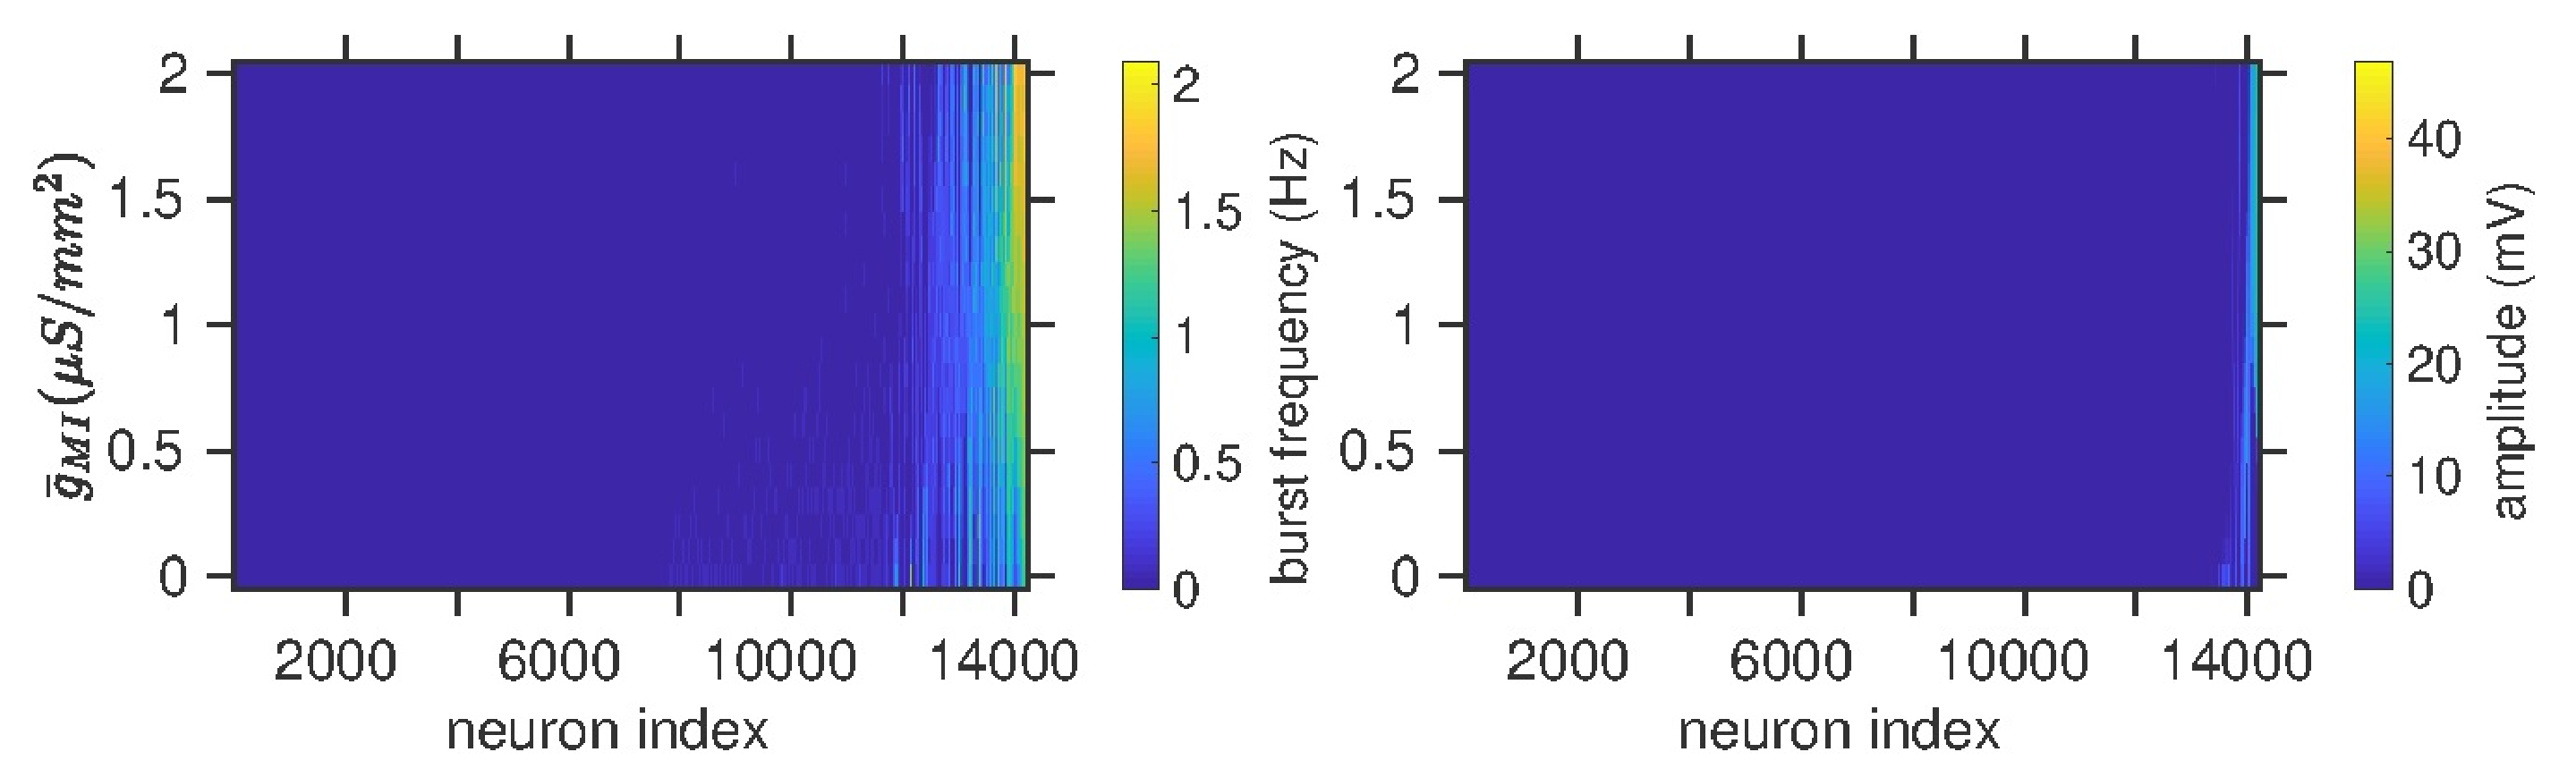
\includegraphics[width=1.0\linewidth]{gfx/prinz-models/prinz}
	\caption[Database models with modulatory input]{Database models without \acs{INa} or \acs{ICaT} with modulatory input respond over a small range of maximal conductance. Most database models do not respond to modulatory input. A subset increase in frequency and amplitude (peak voltage - trough voltage). Models are sorted by mean metric value.}
	\label{fig:prinzburstingmodelsnavcatswensen}
\end{figure}

\begin{figure}[h]
	\centering
	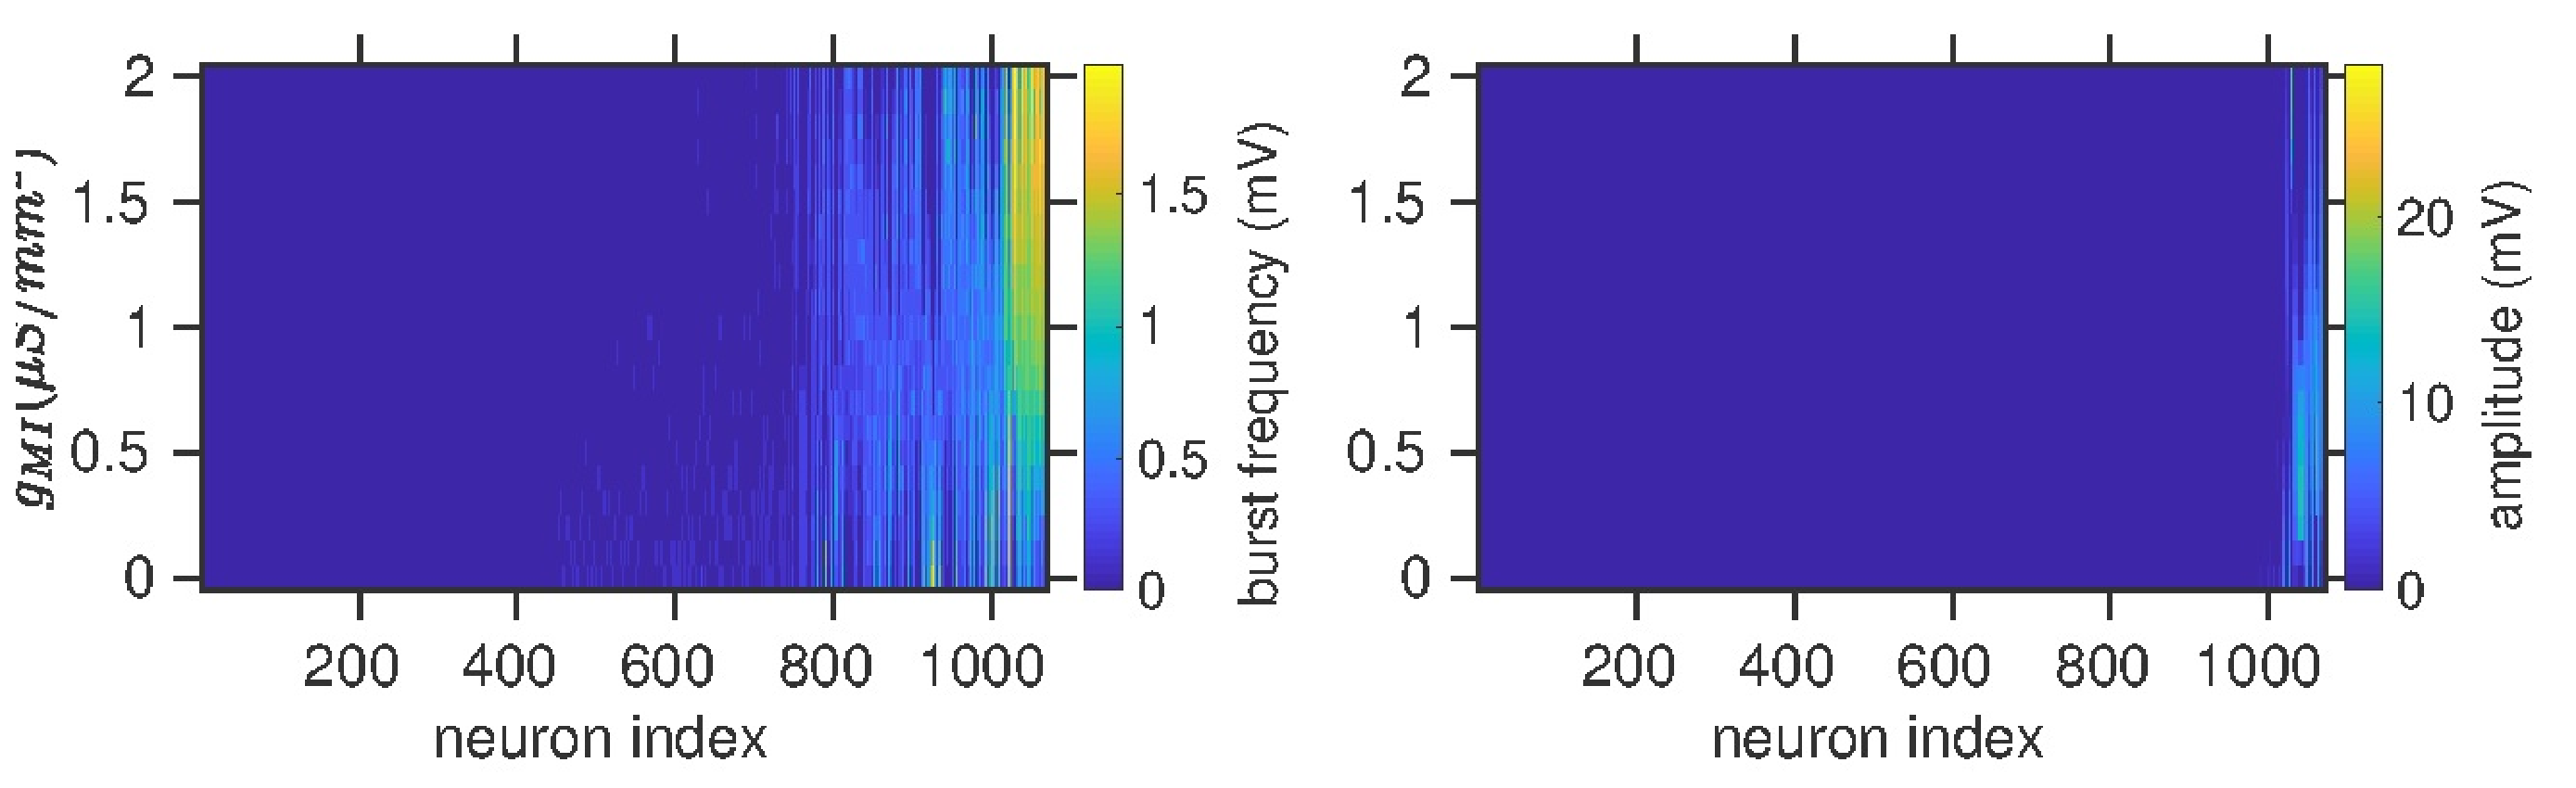
\includegraphics[width=1.0\linewidth]{gfx/prinz-models/prinz_excised}
	\caption[Responsive database models with modulatory input]{A subset of database models with \acs{INa} or \acs{ICaT} were responsive to modulatory input. The 1000 models with the greatest change in frequency and amplitude were plotted with updated color scaling. Models are sorted by mean metric value.}
	\label{fig:prinzburstingmodelsnavcatexcisedswensen}
\end{figure}

\begin{figure}
	\centering
	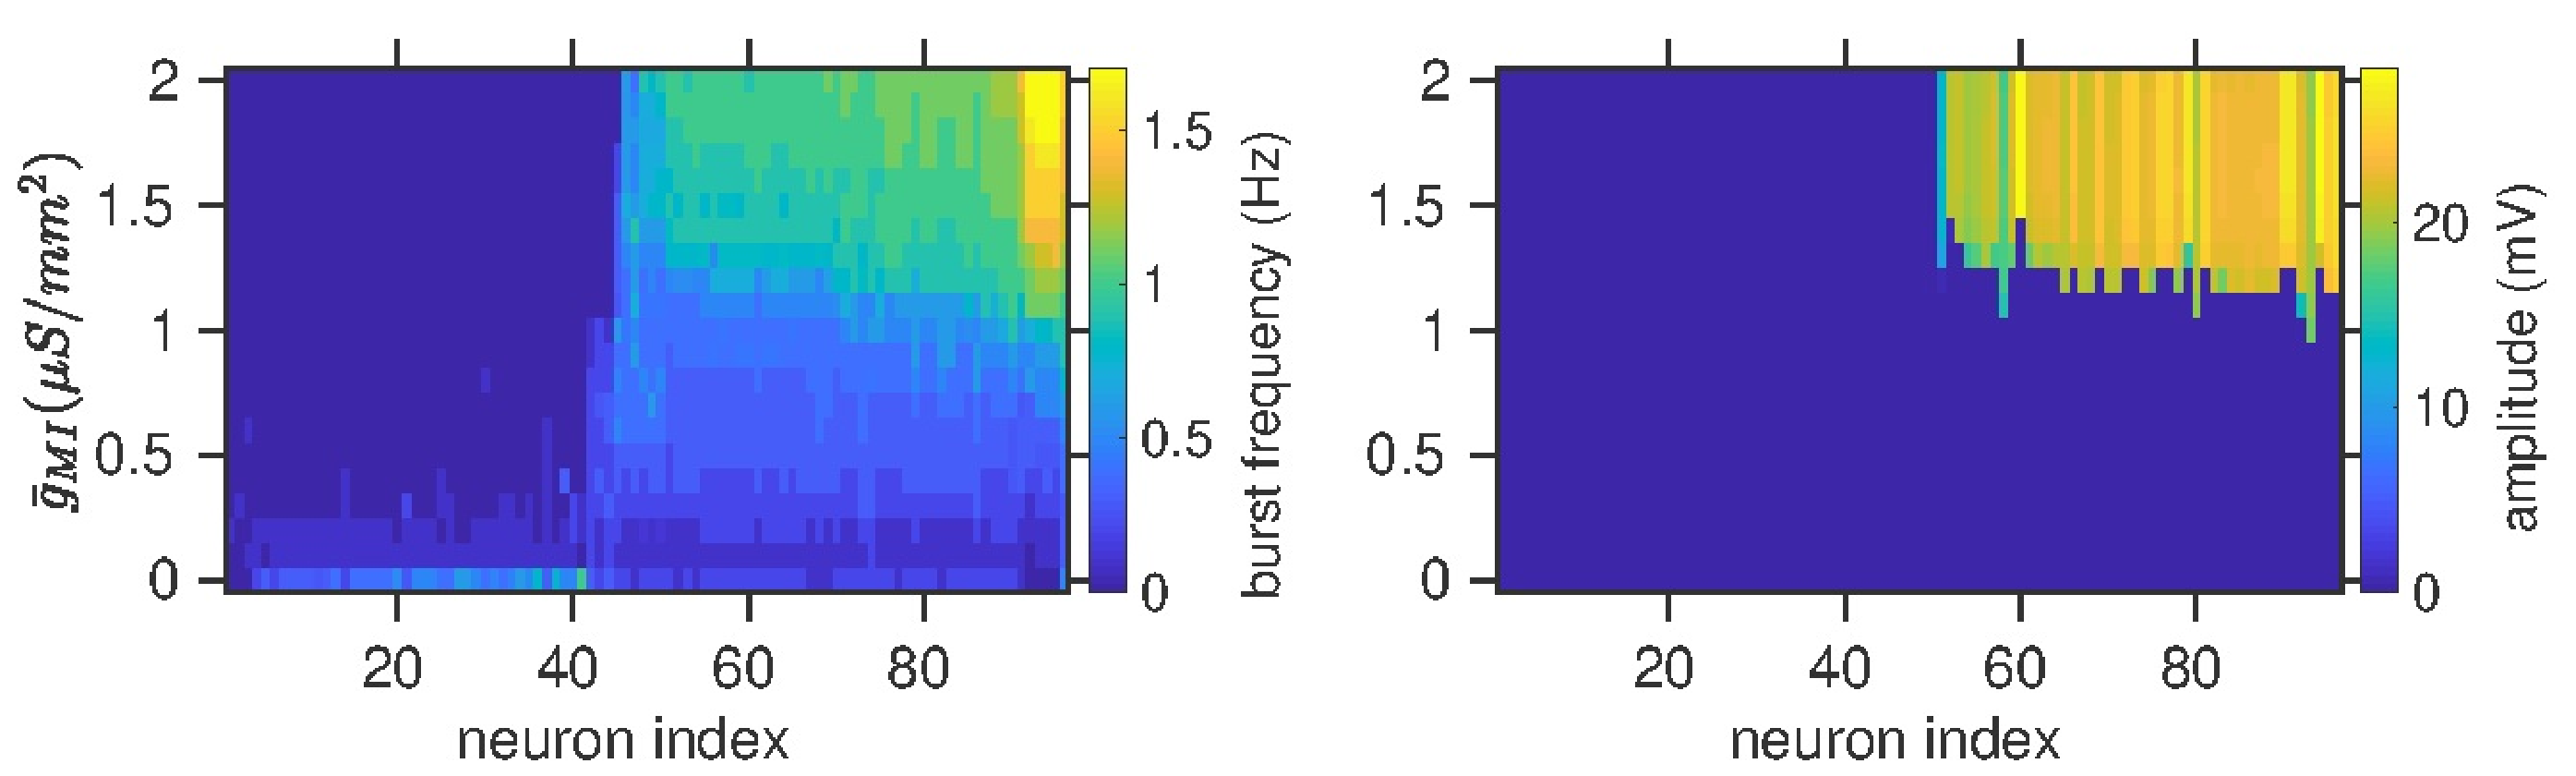
\includegraphics[width=1.0\linewidth]{gfx/prinz-models/prinz_optimized}
	\caption[Optimized database models increase in frequency and amplitude]{Models optimized for a graded increase in frequency and amplitude under increasing modulatory input experience frequency as a graded transition and amplitude as a switch between quiescence and high amplitude. Optimized models display graded increase in burst frequency as the maximal conductance of modulatory input increases. Amplitude increases sharply during a transitional state as maximal conductance of \acs{IMI} increases. Models are sorted by mean metric value.}
	\label{fig:figprinzburstingttxcatnoscgmiswensenexprosim3}
\end{figure}

\begin{figure}
	\centering
	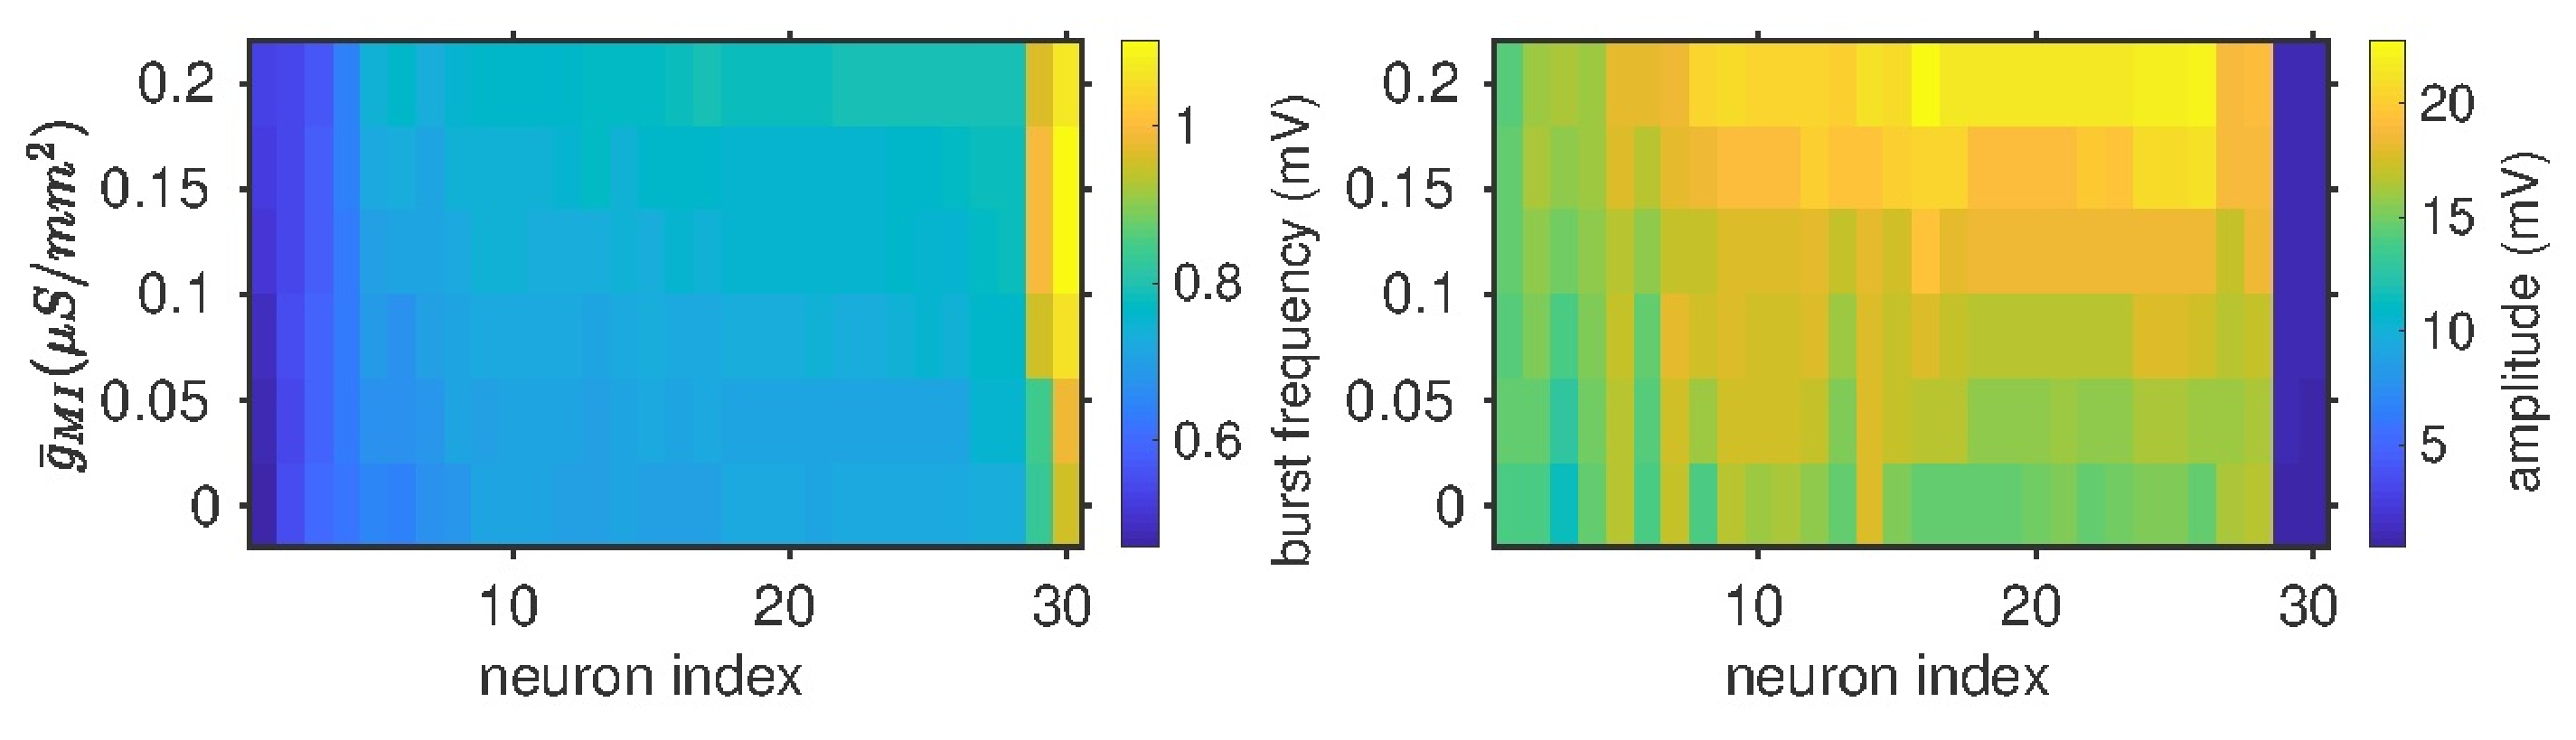
\includegraphics[width=1.0\linewidth]{gfx/prinz-models/plot_optim_AB_graded}
	\caption[Optimized database models smoothly increase in frequency and amplitude]{Models optimized for a graded increase in burst frequency and amplitude over increasing modulatory input. Modulatory input increases the amplitude of slow-wave oscillations by increasing the peak voltage. In these models, the duty cycle remains constant and the frequency increases.}
	\label{fig:plotoptimabgraded}
\end{figure}

